% Options for packages loaded elsewhere
\PassOptionsToPackage{unicode}{hyperref}
\PassOptionsToPackage{hyphens}{url}
%
\documentclass[
]{article}
\usepackage{amsmath,amssymb}
\usepackage{lmodern}
\usepackage{iftex}
\ifPDFTeX
  \usepackage[T1]{fontenc}
  \usepackage[utf8]{inputenc}
  \usepackage{textcomp} % provide euro and other symbols
\else % if luatex or xetex
  \usepackage{unicode-math}
  \defaultfontfeatures{Scale=MatchLowercase}
  \defaultfontfeatures[\rmfamily]{Ligatures=TeX,Scale=1}
\fi
% Use upquote if available, for straight quotes in verbatim environments
\IfFileExists{upquote.sty}{\usepackage{upquote}}{}
\IfFileExists{microtype.sty}{% use microtype if available
  \usepackage[]{microtype}
  \UseMicrotypeSet[protrusion]{basicmath} % disable protrusion for tt fonts
}{}
\makeatletter
\@ifundefined{KOMAClassName}{% if non-KOMA class
  \IfFileExists{parskip.sty}{%
    \usepackage{parskip}
  }{% else
    \setlength{\parindent}{0pt}
    \setlength{\parskip}{6pt plus 2pt minus 1pt}}
}{% if KOMA class
  \KOMAoptions{parskip=half}}
\makeatother
\usepackage{xcolor}
\IfFileExists{xurl.sty}{\usepackage{xurl}}{} % add URL line breaks if available
\IfFileExists{bookmark.sty}{\usepackage{bookmark}}{\usepackage{hyperref}}
\hypersetup{
  pdftitle={Relatório trabalho prático 3},
  pdfauthor={César A. Galvão 19/0011572; Gabriela Carneiro 18/0120816},
  hidelinks,
  pdfcreator={LaTeX via pandoc}}
\urlstyle{same} % disable monospaced font for URLs
\usepackage[margin=1in]{geometry}
\usepackage{color}
\usepackage{fancyvrb}
\newcommand{\VerbBar}{|}
\newcommand{\VERB}{\Verb[commandchars=\\\{\}]}
\DefineVerbatimEnvironment{Highlighting}{Verbatim}{commandchars=\\\{\}}
% Add ',fontsize=\small' for more characters per line
\usepackage{framed}
\definecolor{shadecolor}{RGB}{248,248,248}
\newenvironment{Shaded}{\begin{snugshade}}{\end{snugshade}}
\newcommand{\AlertTok}[1]{\textcolor[rgb]{0.94,0.16,0.16}{#1}}
\newcommand{\AnnotationTok}[1]{\textcolor[rgb]{0.56,0.35,0.01}{\textbf{\textit{#1}}}}
\newcommand{\AttributeTok}[1]{\textcolor[rgb]{0.77,0.63,0.00}{#1}}
\newcommand{\BaseNTok}[1]{\textcolor[rgb]{0.00,0.00,0.81}{#1}}
\newcommand{\BuiltInTok}[1]{#1}
\newcommand{\CharTok}[1]{\textcolor[rgb]{0.31,0.60,0.02}{#1}}
\newcommand{\CommentTok}[1]{\textcolor[rgb]{0.56,0.35,0.01}{\textit{#1}}}
\newcommand{\CommentVarTok}[1]{\textcolor[rgb]{0.56,0.35,0.01}{\textbf{\textit{#1}}}}
\newcommand{\ConstantTok}[1]{\textcolor[rgb]{0.00,0.00,0.00}{#1}}
\newcommand{\ControlFlowTok}[1]{\textcolor[rgb]{0.13,0.29,0.53}{\textbf{#1}}}
\newcommand{\DataTypeTok}[1]{\textcolor[rgb]{0.13,0.29,0.53}{#1}}
\newcommand{\DecValTok}[1]{\textcolor[rgb]{0.00,0.00,0.81}{#1}}
\newcommand{\DocumentationTok}[1]{\textcolor[rgb]{0.56,0.35,0.01}{\textbf{\textit{#1}}}}
\newcommand{\ErrorTok}[1]{\textcolor[rgb]{0.64,0.00,0.00}{\textbf{#1}}}
\newcommand{\ExtensionTok}[1]{#1}
\newcommand{\FloatTok}[1]{\textcolor[rgb]{0.00,0.00,0.81}{#1}}
\newcommand{\FunctionTok}[1]{\textcolor[rgb]{0.00,0.00,0.00}{#1}}
\newcommand{\ImportTok}[1]{#1}
\newcommand{\InformationTok}[1]{\textcolor[rgb]{0.56,0.35,0.01}{\textbf{\textit{#1}}}}
\newcommand{\KeywordTok}[1]{\textcolor[rgb]{0.13,0.29,0.53}{\textbf{#1}}}
\newcommand{\NormalTok}[1]{#1}
\newcommand{\OperatorTok}[1]{\textcolor[rgb]{0.81,0.36,0.00}{\textbf{#1}}}
\newcommand{\OtherTok}[1]{\textcolor[rgb]{0.56,0.35,0.01}{#1}}
\newcommand{\PreprocessorTok}[1]{\textcolor[rgb]{0.56,0.35,0.01}{\textit{#1}}}
\newcommand{\RegionMarkerTok}[1]{#1}
\newcommand{\SpecialCharTok}[1]{\textcolor[rgb]{0.00,0.00,0.00}{#1}}
\newcommand{\SpecialStringTok}[1]{\textcolor[rgb]{0.31,0.60,0.02}{#1}}
\newcommand{\StringTok}[1]{\textcolor[rgb]{0.31,0.60,0.02}{#1}}
\newcommand{\VariableTok}[1]{\textcolor[rgb]{0.00,0.00,0.00}{#1}}
\newcommand{\VerbatimStringTok}[1]{\textcolor[rgb]{0.31,0.60,0.02}{#1}}
\newcommand{\WarningTok}[1]{\textcolor[rgb]{0.56,0.35,0.01}{\textbf{\textit{#1}}}}
\usepackage{graphicx}
\makeatletter
\def\maxwidth{\ifdim\Gin@nat@width>\linewidth\linewidth\else\Gin@nat@width\fi}
\def\maxheight{\ifdim\Gin@nat@height>\textheight\textheight\else\Gin@nat@height\fi}
\makeatother
% Scale images if necessary, so that they will not overflow the page
% margins by default, and it is still possible to overwrite the defaults
% using explicit options in \includegraphics[width, height, ...]{}
\setkeys{Gin}{width=\maxwidth,height=\maxheight,keepaspectratio}
% Set default figure placement to htbp
\makeatletter
\def\fps@figure{htbp}
\makeatother
\setlength{\emergencystretch}{3em} % prevent overfull lines
\providecommand{\tightlist}{%
  \setlength{\itemsep}{0pt}\setlength{\parskip}{0pt}}
\setcounter{secnumdepth}{5}
\usepackage{helvet} \renewcommand\familydefault{\sfdefault}
\usepackage{booktabs}
\usepackage{longtable}
\usepackage{array}
\usepackage{multirow}
\usepackage{wrapfig}
\usepackage{float}
\usepackage{colortbl}
\usepackage{pdflscape}
\usepackage{tabu}
\usepackage{threeparttable}
\usepackage{threeparttablex}
\usepackage[normalem]{ulem}
\usepackage{makecell}
\usepackage{xcolor}
\ifLuaTeX
  \usepackage{selnolig}  % disable illegal ligatures
\fi

\title{Relatório trabalho prático 3}
\author{César A. Galvão 19/0011572 \and Gabriela Carneiro 18/0120816}
\date{21 de August de 2022}

\begin{document}
\maketitle

\newpage{}

{
\setcounter{tocdepth}{3}
\tableofcontents
}
\let\oldsection\section
\renewcommand\section{\clearpage\oldsection}

\hypertarget{introduuxe7uxe3o}{%
\section{Introdução}\label{introduuxe7uxe3o}}

O método de variáveis antitéticas é uma técnica para redução de
variância usado no método de Monte Carlo. A simplicidade do método
sugere que ele pode ser uma ferramenta poderosa para a redução da
variância, mas poucas aplicações bem sucedidas de sua implementação
foram reportadas. A ideia é obter duas estimativas correlacionadas
negativamente para a média \(\mu = \frac{1}{2}(\mu_2 + \mu_1)\), notando
que a estimativa para a variância é reduzida por um termo de
covariância.\footnote{Milgram, M.S. (2001). On the Use of Antithetic
  Variates. In: Kling, A., Baräo, F.J.C., Nakagawa, M., Távora, L., Vaz,
  P. (eds) Advanced Monte Carlo for Radiation Physics, Particle
  Transport Simulation and Applications. Springer, Berlin, Heidelberg.
  \url{https://doi.org/10.1007/978-3-642-18211-2_29}}

Utilizando uma amostra aleatória, um estimador para um para a quantidade
de interesse \(<g> = \int^1_0g(x)p(x)dx\) é convencionalmente obtido.
Introduzindo \(sigma^2\), a variância de \(g(x)\),

\begin{align}
  \sigma^2 \equiv \int_0^1 \{ g(x) - <g>\}^2 \, p(x) \, dx = \int^1_0 g(x)^2 p(x) \, dx - <g>^2 \equiv <g^2> - <g>^2.
\end{align}

Um estimador para \(sigma^2\), a variância amostral, pode ser obtida
avaliando

\begin{align}
  s^2 \equiv \left( \frac{1}{N-1} \right) \sum\limits^N_{i=1}(t_i \mu)^2, 
\end{align}

e

\begin{align}
s^2_\mu = s^2/N \label{13}
\end{align}

a variância da média.

Se \(mu\) for calculada muitas vezes, a estimativa \(mu_i\) iria
coletivamente formar uma distribuição sobre a média das médias
\(\bar{\mu}\), sendo \(s^2_\mu\) um estimador da variância
\(var(\bar{\mu})\) dessa segunda distribuição. Reconhecendo que a
igualdade em (\ref{13}) é obtida assumindo que as amostras \(t_i\) são
independentes, se algum de seus subconjuntos são correlacionados, então,
na verdade

\begin{align}
s^2_\mu = \frac{1}{N} \left[ s^2 + 2 \sum\limits_{p<q} Cov(t_p, t_q) \right].
\end{align}

Se a correlação existe, \(s^2_\mu\) conforme computado por (\ref{13})
será uma estimativa pobre para a variável \(var(\mu)\). Além disso,
deve-se fazer uma distinção entre a redução da variância amostral e a
redução da variância real, sem a qual, é possível observar reduções
falsas ou paradoxais na variância. Dessa forma, três cenários podem ser
observados:

\begin{itemize}
\tightlist
\item
  Redução de \(\sigma^2\) e de \(s^2_\mu\) (caso A), que é o objetivo;
\item
  Redução de \(\sigma^2\), mas não de \(s^2_\mu\) (caso B);
\item
  Redução de \(s^2_\mu\), mas não de \(\sigma^2\) (caso C).
\end{itemize}

\hypertarget{muxe9todo}{%
\section{Método}\label{muxe9todo}}

Foram utilizadas as funções de geração de amostras das variáveis
aleatórias Uniforme e Normal -- esta podendo ser gerada pelos métodos da
rejeição e polar. Apenas a última foi utilizada para a geração da v.a.
normal.

Para cada elemento de \(Z = \{ z_i \in (0, 0.01, 0.02, ..., 3.99) \}\),
foi calculada a probabilidade acumulada da distribuição Normal pelos
métodos de variável antitética e por estimador de regressão.

Para o primeiro método de estimação, utiliza-se \(E(I)=p\), pois
\(I \sim Bernoulli(p)\). Calcula-se portanto
\(\sum\limits_{k = 1}^{n} \frac{i_{k}}{n}\), caso em que a variância
seria \(\frac{\bar{i}(1- \bar{i})}{n}\).

Para o segundo método, utiliza-se \(I = aZ + b\), calcula-se \(p\) por
\(\hat{a} E(Z) + \hat{b} = \hat{b}\). A variância é
\(\frac{\sigma^2}{n}\), em que \(\sigma^2\) é a variância dos resíduos
do modelo de regressão.

Em seguida, foram calculados os erros de estimação em relação à função
implementada \texttt{pnorm()}. Por fim, são comparadas as variâncias
entre os métodos.

\hypertarget{resultados}{%
\section{Resultados}\label{resultados}}

\hypertarget{avaliauxe7uxe3o-dos-erros}{%
\subsection{Avaliação dos erros}\label{avaliauxe7uxe3o-dos-erros}}

Nota-se pelos gráficos a seguir que os erros para ambos os métodos
seguem uma mesma tendência, se aproximando de zero na medida em que os
valores de Z crescem.

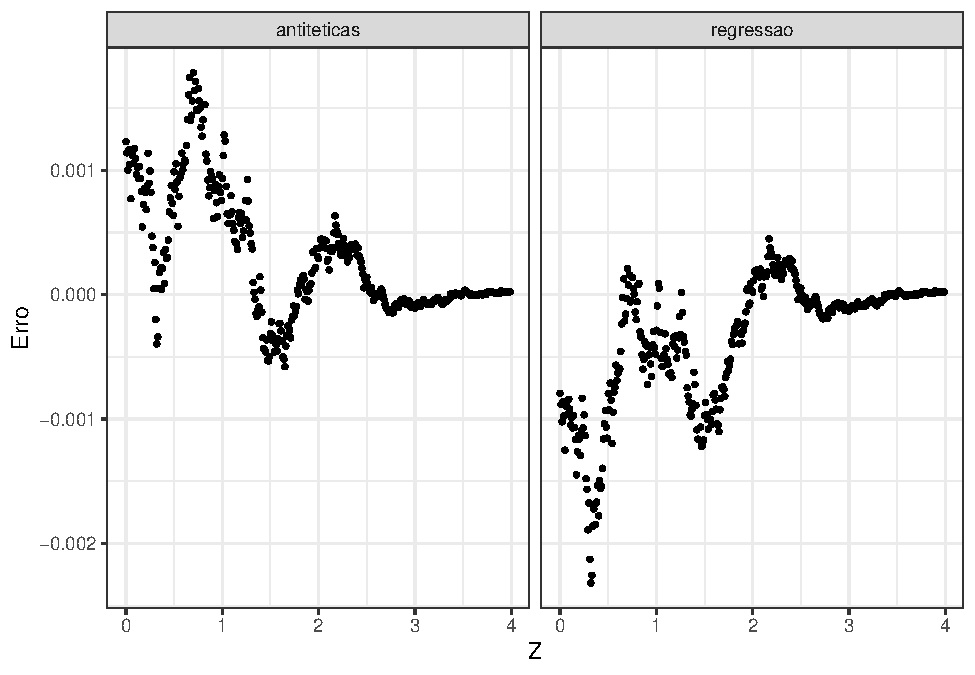
\includegraphics[width=0.6\linewidth]{tp-3_files/figure-latex/calculo-acumuladas-1}

Finalmente, compara-se as variâncias dos métodos de variáveis
antitéticas e de regressão. Observa-se que quanto maior o valor de Z,
mais próximo de 1 fica a razão entre as variâncias. Para pequenos
valores de Z, portanto, a variância do método de variáveis antitéticas é
maior.

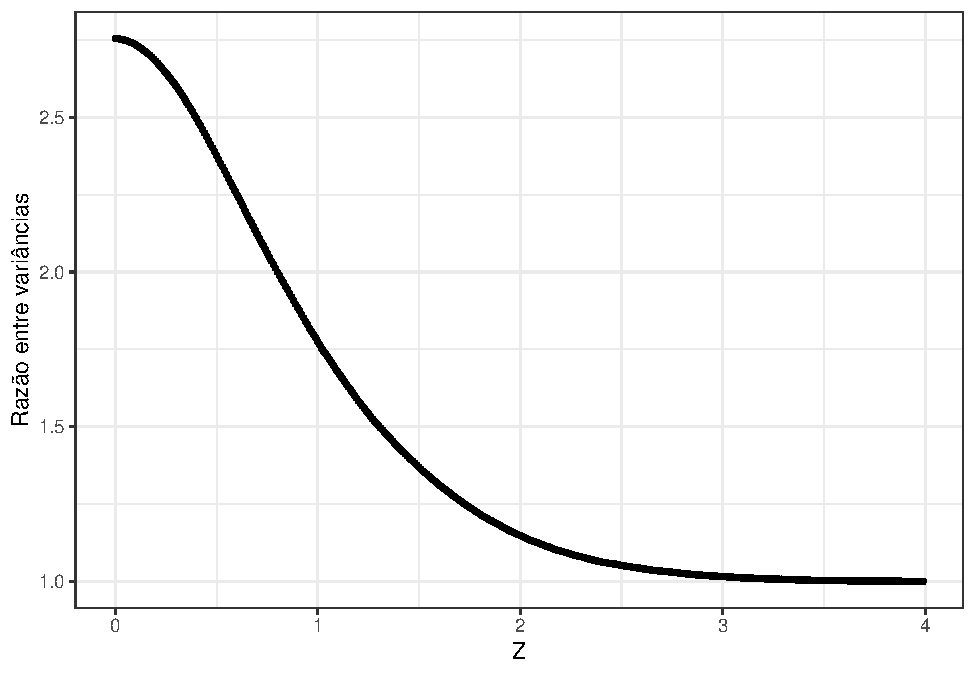
\includegraphics[width=0.6\linewidth]{tp-3_files/figure-latex/compara-variancias-1}

\hypertarget{cuxf3digo}{%
\section{Código}\label{cuxf3digo}}

\begin{Shaded}
\begin{Highlighting}[]
\NormalTok{uniforme }\OtherTok{\textless{}{-}} \ControlFlowTok{function}\NormalTok{(n)\{}
  
\NormalTok{  x }\OtherTok{\textless{}{-}} \FunctionTok{c}\NormalTok{()}
  
\NormalTok{  a }\OtherTok{\textless{}{-}} \DecValTok{16807}
\NormalTok{  m }\OtherTok{\textless{}{-}} \DecValTok{2}\SpecialCharTok{\^{}}\DecValTok{31} \SpecialCharTok{{-}}\DecValTok{1}
  
  \CommentTok{\# se tem o arquivo com seed, pega o seed k do arquivo}
  \CommentTok{\# Se nao tiver arquivo, gera o arquivo e escreve o seed}
  \CommentTok{\# seed começa com o relogio}
  \CommentTok{\# Os que extrapolarem inserir no arquivo}
  
  \ControlFlowTok{if}\NormalTok{ (}\FunctionTok{file.exists}\NormalTok{(}\StringTok{"../trabalho pratico 2/seeds.Rdata"}\NormalTok{))\{}
\NormalTok{    y }\OtherTok{\textless{}{-}} \FunctionTok{readRDS}\NormalTok{(}\StringTok{"../trabalho pratico 2/seeds.Rdata"}\NormalTok{)}
\NormalTok{  \} }\ControlFlowTok{else}\NormalTok{ \{}
\NormalTok{    y }\OtherTok{\textless{}{-}} \FunctionTok{as.numeric}\NormalTok{(}\FunctionTok{Sys.time}\NormalTok{())}
\NormalTok{  \}}
  
  \ControlFlowTok{for}\NormalTok{ (i }\ControlFlowTok{in} \DecValTok{1}\SpecialCharTok{:}\NormalTok{n)\{}
\NormalTok{    y }\OtherTok{\textless{}{-}}\NormalTok{ (a}\SpecialCharTok{*}\NormalTok{y)}\SpecialCharTok{\%\%}\NormalTok{m}
\NormalTok{    x[i] }\OtherTok{\textless{}{-}}\NormalTok{ y}\SpecialCharTok{/}\NormalTok{m}
\NormalTok{  \}}
  
  \CommentTok{\#guardar o ultimo y num arquivo}
  \FunctionTok{saveRDS}\NormalTok{(y, }\StringTok{"../trabalho pratico 2/seeds.Rdata"}\NormalTok{)}
  
  \FunctionTok{return}\NormalTok{(x)}
\NormalTok{\}}

\NormalTok{geranormal }\OtherTok{\textless{}{-}} \ControlFlowTok{function}\NormalTok{(metodo)\{}
  \ControlFlowTok{if}\NormalTok{ (metodo }\SpecialCharTok{==} \StringTok{"rejeicao"}\NormalTok{)\{}
\NormalTok{    y }\OtherTok{\textless{}{-}} \FunctionTok{geraexp}\NormalTok{(}\AttributeTok{n =} \DecValTok{1}\NormalTok{, }\AttributeTok{lambda =} \DecValTok{1}\NormalTok{)}
\NormalTok{    u }\OtherTok{\textless{}{-}} \FunctionTok{uniforme}\NormalTok{(}\DecValTok{1}\NormalTok{)}
    \ControlFlowTok{while}\NormalTok{(u }\SpecialCharTok{\textgreater{}} \FunctionTok{exp}\NormalTok{(}\SpecialCharTok{{-}}\NormalTok{(y}\DecValTok{{-}1}\NormalTok{)}\SpecialCharTok{\^{}}\DecValTok{2}\NormalTok{)}\SpecialCharTok{/}\DecValTok{2}\NormalTok{)\{}
\NormalTok{      u }\OtherTok{\textless{}{-}} \FunctionTok{uniforme}\NormalTok{(}\DecValTok{1}\NormalTok{)}
\NormalTok{      y }\OtherTok{\textless{}{-}} \FunctionTok{geraexp}\NormalTok{(}\AttributeTok{n =} \DecValTok{1}\NormalTok{, }\AttributeTok{lambda =} \DecValTok{1}\NormalTok{)}
\NormalTok{    \}}
\NormalTok{    modZ }\OtherTok{\textless{}{-}} \FunctionTok{abs}\NormalTok{(y)}
    
    \ControlFlowTok{if}\NormalTok{(}\FunctionTok{uniforme}\NormalTok{(}\DecValTok{1}\NormalTok{) }\SpecialCharTok{\textless{}=} \FloatTok{0.5}\NormalTok{)\{}
\NormalTok{      Z }\OtherTok{\textless{}{-}}\NormalTok{ modZ}
\NormalTok{    \} }\ControlFlowTok{else}\NormalTok{ \{}
\NormalTok{      Z }\OtherTok{\textless{}{-}} \SpecialCharTok{{-}}\NormalTok{modZ}
\NormalTok{    \}}
    \FunctionTok{return}\NormalTok{(Z)}
\NormalTok{  \}}
  
  \ControlFlowTok{if}\NormalTok{(metodo }\SpecialCharTok{==} \StringTok{"polar"}\NormalTok{)\{}
\NormalTok{    v1 }\OtherTok{\textless{}{-}}\NormalTok{ (}\DecValTok{2}\SpecialCharTok{*}\FunctionTok{uniforme}\NormalTok{(}\DecValTok{1}\NormalTok{)}\SpecialCharTok{{-}}\DecValTok{1}\NormalTok{)}
\NormalTok{    v2 }\OtherTok{\textless{}{-}}\NormalTok{ (}\DecValTok{2}\SpecialCharTok{*}\FunctionTok{uniforme}\NormalTok{(}\DecValTok{1}\NormalTok{)}\SpecialCharTok{{-}}\DecValTok{1}\NormalTok{)}
\NormalTok{    u }\OtherTok{\textless{}{-}}\NormalTok{ v1}\SpecialCharTok{\^{}}\DecValTok{2} \SpecialCharTok{+}\NormalTok{ v2}\SpecialCharTok{\^{}}\DecValTok{2}
    \ControlFlowTok{while}\NormalTok{ (u }\SpecialCharTok{\textgreater{}} \DecValTok{1}\NormalTok{)\{}
\NormalTok{      v1 }\OtherTok{\textless{}{-}}\NormalTok{ (}\DecValTok{2}\SpecialCharTok{*}\FunctionTok{uniforme}\NormalTok{(}\DecValTok{1}\NormalTok{)}\SpecialCharTok{{-}}\DecValTok{1}\NormalTok{)}
\NormalTok{      v2 }\OtherTok{\textless{}{-}}\NormalTok{ (}\DecValTok{2}\SpecialCharTok{*}\FunctionTok{uniforme}\NormalTok{(}\DecValTok{1}\NormalTok{)}\SpecialCharTok{{-}}\DecValTok{1}\NormalTok{)}
\NormalTok{      u }\OtherTok{\textless{}{-}}\NormalTok{ v1}\SpecialCharTok{\^{}}\DecValTok{2} \SpecialCharTok{+}\NormalTok{ v2}\SpecialCharTok{\^{}}\DecValTok{2}
\NormalTok{    \}}
\NormalTok{    x }\OtherTok{\textless{}{-}} \FunctionTok{sqrt}\NormalTok{(}\SpecialCharTok{{-}}\DecValTok{2}\SpecialCharTok{*}\FunctionTok{log}\NormalTok{(u)}\SpecialCharTok{/}\NormalTok{u)}\SpecialCharTok{*}\NormalTok{v1}
\NormalTok{    y }\OtherTok{\textless{}{-}} \FunctionTok{sqrt}\NormalTok{(}\SpecialCharTok{{-}}\DecValTok{2}\SpecialCharTok{*}\FunctionTok{log}\NormalTok{(u)}\SpecialCharTok{/}\NormalTok{u)}\SpecialCharTok{*}\NormalTok{v2}
    \FunctionTok{return}\NormalTok{(}\FunctionTok{list}\NormalTok{(}\AttributeTok{x =}\NormalTok{ x, }\AttributeTok{y =}\NormalTok{ y))}
\NormalTok{  \}}
\NormalTok{\}}

\NormalTok{intervalo }\OtherTok{\textless{}{-}} \FunctionTok{seq}\NormalTok{(}\DecValTok{0}\NormalTok{, }\FloatTok{3.99}\NormalTok{, }\FloatTok{0.01}\NormalTok{)}

\NormalTok{prob\_acum\_z }\OtherTok{\textless{}{-}} \ControlFlowTok{function}\NormalTok{(amostra, z, metodo)\{}
\NormalTok{  j }\OtherTok{\textless{}{-}} \FunctionTok{as.numeric}\NormalTok{(amostra }\SpecialCharTok{\textless{}}\NormalTok{ z)}
  \ControlFlowTok{if}\NormalTok{(metodo}\SpecialCharTok{==}\StringTok{"antitetica"}\NormalTok{)\{}
    \FunctionTok{return}\NormalTok{(}\FunctionTok{data.frame}\NormalTok{(}\StringTok{"z"} \OtherTok{=}\NormalTok{ z, }
                      \StringTok{"p"} \OtherTok{=} \FunctionTok{mean}\NormalTok{(j), }\CommentTok{\#media da va indicadora }
                      \StringTok{"var\_p"}\OtherTok{=} \FunctionTok{mean}\NormalTok{(j)}\SpecialCharTok{*}\NormalTok{(}\DecValTok{1}\SpecialCharTok{{-}}\FunctionTok{mean}\NormalTok{(j))}\SpecialCharTok{/}\FunctionTok{length}\NormalTok{(j))) }\CommentTok{\#p(1{-}p)/n}
\NormalTok{  \}}
  \ControlFlowTok{if}\NormalTok{(metodo}\SpecialCharTok{==}\StringTok{"regressao"}\NormalTok{)\{}
\NormalTok{    reg }\OtherTok{\textless{}{-}} \FunctionTok{lm}\NormalTok{(j }\SpecialCharTok{\textasciitilde{}}\NormalTok{ amostra)}
    \FunctionTok{return}\NormalTok{(}\FunctionTok{data.frame}\NormalTok{(}\StringTok{"z"} \OtherTok{=}\NormalTok{ z,}
                      \StringTok{"p"} \OtherTok{=}\NormalTok{ reg}\SpecialCharTok{$}\NormalTok{coefficients[[}\DecValTok{1}\NormalTok{]], }\CommentTok{\#p = intercepto}
                      \StringTok{"var\_p"}\OtherTok{=} \FunctionTok{var}\NormalTok{(reg}\SpecialCharTok{$}\NormalTok{residuals)}\SpecialCharTok{/}\FunctionTok{length}\NormalTok{(j))) }\CommentTok{\#sigma\^{}2/n}
\NormalTok{  \}}
\NormalTok{\}}

\NormalTok{amostra }\OtherTok{\textless{}{-}} \FunctionTok{c}\NormalTok{()}
\ControlFlowTok{for}\NormalTok{(i }\ControlFlowTok{in} \DecValTok{1}\SpecialCharTok{:}\DecValTok{100000}\NormalTok{)\{ amostra[i] }\OtherTok{\textless{}{-}} \FunctionTok{geranormal}\NormalTok{(}\StringTok{"polar"}\NormalTok{)}\SpecialCharTok{$}\NormalTok{x\}}

\NormalTok{antiteticas }\OtherTok{\textless{}{-}} \FunctionTok{data.frame}\NormalTok{(}\AttributeTok{z =} \DecValTok{0}\NormalTok{, }\AttributeTok{p =} \DecValTok{0}\NormalTok{, }\AttributeTok{var\_p =} \DecValTok{0}\NormalTok{)}
\ControlFlowTok{for}\NormalTok{(i }\ControlFlowTok{in} \DecValTok{1}\SpecialCharTok{:}\FunctionTok{length}\NormalTok{(intervalo))\{antiteticas[i,] }\OtherTok{\textless{}{-}} \FunctionTok{prob\_acum\_z}\NormalTok{(amostra, intervalo[i], }\StringTok{"antitetica"}\NormalTok{)\}}

\NormalTok{regressao }\OtherTok{\textless{}{-}} \FunctionTok{data.frame}\NormalTok{(}\AttributeTok{z =} \DecValTok{0}\NormalTok{, }\AttributeTok{p =} \DecValTok{0}\NormalTok{, }\AttributeTok{var\_p =} \DecValTok{0}\NormalTok{)}
\ControlFlowTok{for}\NormalTok{(i }\ControlFlowTok{in} \DecValTok{1}\SpecialCharTok{:}\FunctionTok{length}\NormalTok{(intervalo))\{regressao[i,] }\OtherTok{\textless{}{-}} \FunctionTok{prob\_acum\_z}\NormalTok{(amostra, intervalo[i], }\StringTok{"regressao"}\NormalTok{)\}}

\NormalTok{erros }\OtherTok{\textless{}{-}} \FunctionTok{data.frame}\NormalTok{(}
\NormalTok{  intervalo, }
  \AttributeTok{antiteticas =}\NormalTok{ antiteticas}\SpecialCharTok{$}\NormalTok{p }\SpecialCharTok{{-}} \FunctionTok{pnorm}\NormalTok{(intervalo),}
  \AttributeTok{regressao =}\NormalTok{ regressao}\SpecialCharTok{$}\NormalTok{p }\SpecialCharTok{{-}} \FunctionTok{pnorm}\NormalTok{(intervalo)}
\NormalTok{) }\SpecialCharTok{\%\textgreater{}\%}
  \FunctionTok{pivot\_longer}\NormalTok{(}\AttributeTok{cols =} \SpecialCharTok{{-}}\NormalTok{intervalo, }\AttributeTok{names\_to =} \StringTok{"tipo"}\NormalTok{, }\AttributeTok{values\_to =} \StringTok{"erro"}\NormalTok{)}

\NormalTok{graf }\OtherTok{\textless{}{-}} \FunctionTok{ggplot}\NormalTok{(erros, }\FunctionTok{aes}\NormalTok{(intervalo, erro))}\SpecialCharTok{+}
  \FunctionTok{geom\_point}\NormalTok{(}\AttributeTok{size =}\NormalTok{ .}\DecValTok{8}\NormalTok{)}\SpecialCharTok{+}
  \FunctionTok{facet\_grid}\NormalTok{(}\SpecialCharTok{\textasciitilde{}}\NormalTok{tipo)}\SpecialCharTok{+}
  \FunctionTok{labs}\NormalTok{(}\AttributeTok{x =} \StringTok{"Z"}\NormalTok{, }\AttributeTok{y =} \StringTok{"Erro"}\NormalTok{)}\SpecialCharTok{+}
  \FunctionTok{theme\_bw}\NormalTok{()}

\NormalTok{graf}

\FunctionTok{data.frame}\NormalTok{(}\StringTok{"z"} \OtherTok{=}\NormalTok{ antiteticas}\SpecialCharTok{$}\NormalTok{z, }\StringTok{"razao"} \OtherTok{=}\NormalTok{ antiteticas}\SpecialCharTok{$}\NormalTok{var\_p}\SpecialCharTok{/}\NormalTok{regressao}\SpecialCharTok{$}\NormalTok{var\_p) }\SpecialCharTok{\%\textgreater{}\%}
  \FunctionTok{ggplot}\NormalTok{() }\SpecialCharTok{+}
  \FunctionTok{geom\_point}\NormalTok{(}\FunctionTok{aes}\NormalTok{(z, razao), }\AttributeTok{size =}\NormalTok{ .}\DecValTok{8}\NormalTok{) }\SpecialCharTok{+}
  \FunctionTok{labs}\NormalTok{(}\AttributeTok{x =} \StringTok{"Z"}\NormalTok{, }\AttributeTok{y =} \StringTok{"Razão entre variâncias"}\NormalTok{)}\SpecialCharTok{+}
  \FunctionTok{theme\_bw}\NormalTok{()}
\end{Highlighting}
\end{Shaded}


\end{document}
